\chapter{Work environment}
\label{chap:env}

In section \ref{sec:vmclass} we have introduced a classification of Virtual Machine systems.
The work presented in this thesis is restricted to same-ISA System Virtual Machines, where the Virtual Machine Monitor is a type 2 VMM.
In other words, we will deal with VMs that are able to run an arbitrary OS compiled for the host ISA. The guest OS can in turn provide an 
execution environment for many user applications.
Since the VMM is of type 2, it is implemented as a regular process in the host OS, and can make use of all the OS services.
We can therefore access the host physical resources without requiring administrator previleges.

We also restrict our work to VMMs that make use of hardware-based virtualization, because the optimizations we will introduce are
particularly effective in limiting the amount of VM switches between the host world and the guest world. Since these VM switches
are very expensive with hardware virtualization, the performance gain is going to be significant.

\vspace{0.5cm}

While the assumptions made may appear restrictive, they are not at all. The class of VMMs that we consider is extremely 
common in the world of computing. These VMMs are used in datacenters and IT departments for server consolidation, 
application isolation, to provide users/developers with zero-setup computing environments or for other application in which it is not
important that the VM computing environment has a different ISA from the host ISA. Moreover, hardware-based virtualization is generally
the most efficient CPU virtualization technique, and so it's worth focusing on this case.
Several VMM software belonging to the considered class are available. QEMU, VirtualBox, VMWare, Parallels, Windows
Hyper-V or Windows VirtualPC are among the most common examples of this kind of VMMs. These software tools are extremely widespread
and for this reason performance optimizations in these area are certainly useful.

\vspace{0.5cm}

This said, we have chosen the QEMU-KVM Virtual Machine Monitor for implementations and tests, although our optimizations are
relevant to the entire class of VMMs.

A GNU/Linux-based operating system (Archlinux) has been used on the host machine. The guest OS is generally Archlinux, but 
some tests have been performed with FreeBSD as a guest, too. Although Linux is a kernel and not a complete OS, in the following we 
will use  the expression ``Linux OS'' to actually mean ``GNU/Linux-based OS'', for the sake of simplicity.

Since our optimizations concern network performance, we had to choose a network device to work with. The \emph{e1000} class of 
network devices was chosen, since it is emulated by the vast majority of VMMs and supported by the main OSs (Windows, Linux, FreeBSD).


\section{QEMU features}
QEMU (\cite{ref:qemu}, \cite{ref:qemu-paper}) is a free, open source and multi-platform type 2 VMM, that makes use of dynamic translation to
achieve good emulation performance. QEMU-KVM is a QEMU branch that extends the original software to take advantage of hardware-based 
virtualization. Whenever possible, QEMU-KVM uses hardware virtualization in order to execute guest code natively.
In the following we will use the terms QEMU and QEMU-KVM in an interchangeable manner.
At the time of this writing, the QEMU-KVM version number is 1.2.0, and so we will refer to that version.

\vspace{0.5cm}

QEMU is a very flexible tool:
\begin{itemize}
    \item It supports process virtual machines: by means of dynamic translation it can execute on the host OS a single program compiled 
	  for an other ISA. This operating mode is called \emph{User mode emulation}.
	  
    \item It supports system virtual machines: by means of dynamic translation and hardware-assisted virtualization (when possible) it
	  can emulate full computer systems (including common peripherals), supporting unmodified operating systems. This operating
	  mode (which is the one we are interested in) is called \emph{Full system emulation}.
	  
    \item It supports various architectures, including  IA-32 (x86), x86-64, MIPS R4000, Sun's SPARC sun4m, Sun's SPARC sun4u,
	  ARM development boards (Integrator/CP and Versatile/PB), SH4 SHIX board, PowerPC,
	  ETRAX CRIS and MicroBlaze architectures.
	  
    \item It can emulate Symmetric Multiprocessing Systems (SMP), making use of all the CPUs that are present on the 
	  host system.
	  
    \item It is able to emulate various peripherals, such as hard disks, CD-ROM drives, network cards, audio interfaces, 
	  or USB devices.
	  
    \item Like similar hypervisors, it is able to provide its VM with network connectivity. The way this can be done will be
	  presented in section \ref{sec:qemunet}.
	  
    \item It does not normally require administrative rights to run. In our experiments administrative rights won't be
	  necessary.
\end{itemize}

QEMU is able to emulate the e1000 class of PCI network adapters\footnote{To be more precise, the emulated hardware exposes
to the guest OS the PCI device ID of the 82540EM model.}, as well as other network devices (RTL8139C+, i8255x (PRO100), 
NE2000 (RTL8029), AMD PCNET II (Am79C7070a)).

Moreover, QEMU supports the \emph{Virtio} framework, that exposes a paravirtualized network device, \emph{virtio-net}, intended 
to be used for high performance networking. The Virtio paravirtualized soution will be analized in chapter \ref{cha:paravirt}.



\section{QEMU internal architecture}
In this section we will illustrate those details of QEMU implementation that is necessary understand in order to implement our
optimizations.

\subsection{QEMU event-loop}
\label{sec:qemuel}
QEMU is an event-loop based software, implemented as a single-process multi-threaded application. 
One thread, referred to as \emph{IOThread}, executes the event-loop, waiting for new events to occur\footnote{This is 
implemented in \texttt{main-loop.c}}.
The waiting routine is a \texttt{select()} system call, which is not the most efficient choice on Unix-like
systems\footnote{ \texttt{poll()}, and specially Linux \texttt{epoll()} or BSD \texttt{kqueue()} are more efficient.},
but is more portable across different platforms.

\vspace{0.5cm}

The file descriptors associated with the \texttt{select()} can be associated to regular files, sockets, device files (such as TAP 
devices), or even special in-kernel objects, such as POSIX timers, signals and eventfds. These file descriptors are used by QEMU to let
the VM communicate with the host, and possibly with the rest of the Internet. In other words, they are used for performing the I/O 
operations requested by the VM. Of course the guest OS still performs I/O operations accessing I/O ports or memory-mapped I/O (MMIO) in 
its physical address space and is unaware of being emulated.

\vspace{0.5cm}

The QEMU core codebase offers to the QEMU developer an API that can be used to implement devices emulators.
In particular, the API provides two useful abstractions: the QEMUTimer and the QEMUBH. 

QEMUTimers are one-shot absolute timers, that can be 
used to execute a callback function at a certain point of time in the future. The callback is always executed by the IOThread, when this
recognizes that the deadline has been passed. The QEMUTimers are supported
by the Linux OS with a single one-shot relative POSIX timer\footnote{Similar mechanisms are used in other OS, or if POSIX timers are not
available under the Linux OS.}, which is always (re)armed to expire - waking up the event-loop - at
the earliest deadline. The expiration check for QEMUTimers is done at the end of each event-loop iteration, even if the event-loop was 
waken up for a reason different from the POSIX timer expiration. In the current implementation, moreover, every time the POSIX timer
is rearmed, the relative deadline is forced to be greater or equal that 250 $\mu$s\footnote{For more information about the QEMUTimer
interface and implementation, refer to the file \texttt{qemu-timer.c} in the QEMU project root directory.}.

\vspace{0.5cm}

QEMUBH is the QEMU abstraction of the \emph{bottom half} concept, widely used in OS drivers implementation. A QEMUBH can be seen as
a QEMUTimer that expires as soon as possible. In practice when a QEMUBH is scheduled the event-loop is notified, so that it
wakes up (or finishes the current iteration and begins another iteration) and executes all the callbacks of currently scheduled QEMUBHs.
Therefore the QEMUBH callbacks are always executed by the IOThread, similarly to the QEMUTimer callbacks\footnote{For more information
about the QEMUBH interface and implementation, refer to the files \texttt{qemu-aio.h} and \texttt{async.c} in the QEMU project
root directory}. This feature is very important in terms of parallelism, as will be clear in the following chapters.

\subsection{VCPU Threads}
While executing the event-loop, the IOThread handles all the interactions between the VM and the external world.
The guest code, however, is executed by one or more threads, that we will call \emph{VCPU threads}. In the current implementation QEMU
creates as many VCPU threads as the number of SMP processors specified by the QEMU user.
When using hardware-based virtualization (we made this assumption at the beginning of this chapter), a VCPU thread continuously
switch between the VM mode and the normal mode (see section \ref{sec:hbv}).

\vspace{0.5cm}

When the VCPU tries to execute an I/O operation, accessing I/O ports or MMIO, a VMExit happens. A VMExit also occurs when an interrupt
is delivered to a VCPU. There could be other type of events that cause a VMExit, but we are not interested in them.
On a VMExit the VCPU stops executing guest
code and starts executing QEMU code, in order to handle, if necessary, the event that caused the VMExit.
After the event has been handled, the VPCU executes a VMEnter and continues to run the guest code from the point where it was interrupted.

\vspace{0.5cm}

Since multiple threads are involved, and all of them - IOThread included - can access the shared structures used by the emulator
(e.g. the structures employed to implement the virtual devices), mutual exclusion is required. In the current implementation the
mutual exclusion is guaranteed by a single big-lock, called the \texttt{iothread lock}.

Therefore, everytime a VCPU VMExits, it has to acquire the \texttt{iothread lock} before it can handle the event. After the event has been
handled, the VPCU thread release the \texttt{iothread lock} and executes a VMEnter instruction.
Similarly, the IOthread has to acquire the \texttt{iothread lock} every time it wakes up for event handling, and release the lock
only when the event-loop iteration terminates.

Putting all together, the figure \ref{fig:qemuthreads} depicts the QEMU thread scheme.

\begin{figure}[bt]
\centering
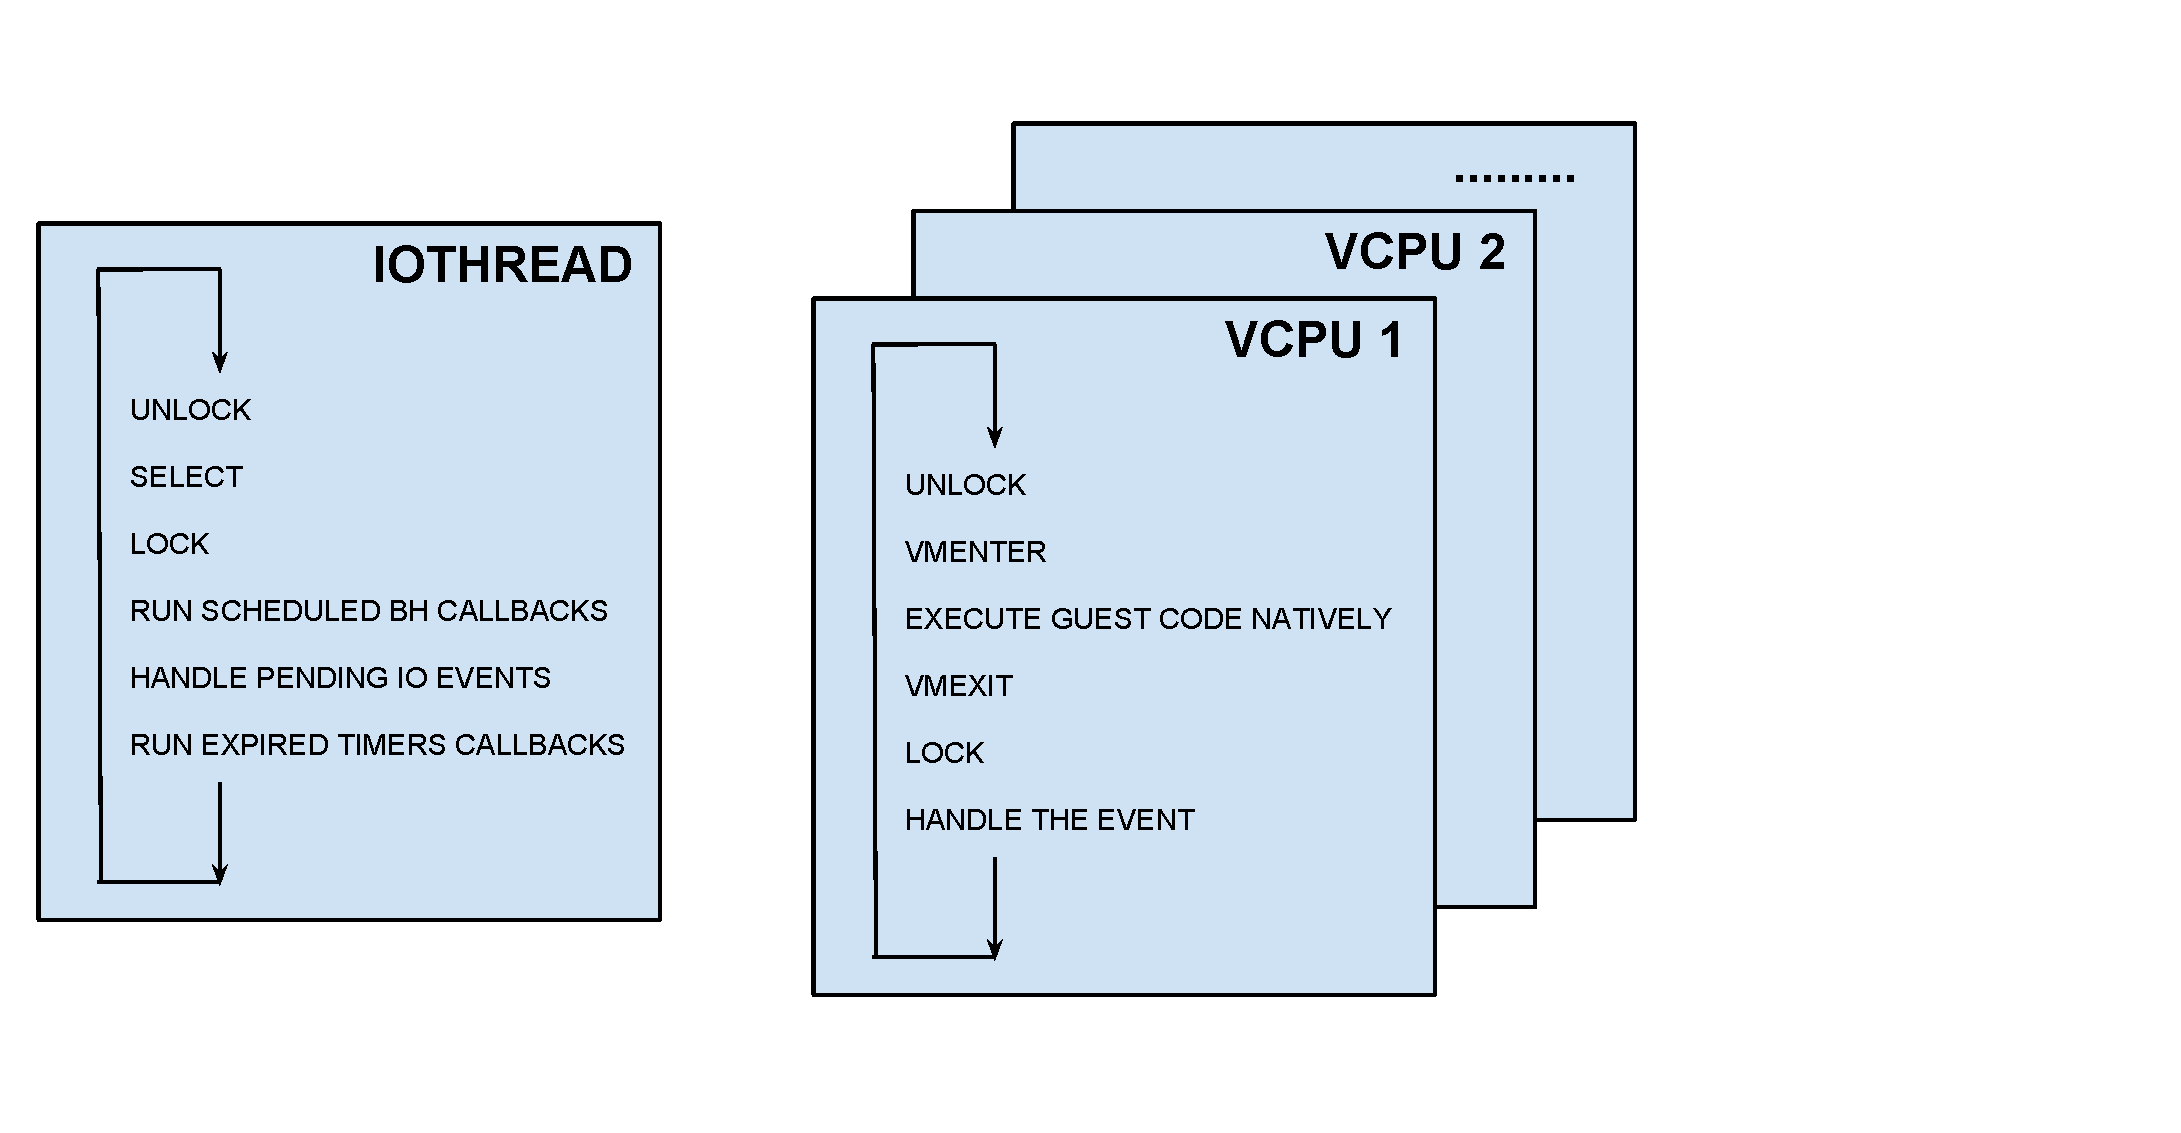
\includegraphics[scale = 0.45]{qemu-threads.pdf}
\caption{QEMU thread scheme.}
\label{fig:qemuthreads}
\end{figure}



\subsection{Networking architectures}
\label{sec:qemunet}
When running a VM it is of fundamental importance to make possible for the guest to communicate with the outside world using the
networking infrastructure, otherwise the VM itself would be an useless computing box.

Since the VM it's a software entity, however, it isn't connected to any real network. Therefore the hypervisor has to provide some
form of network infrastructure virtualization, so that the guest OS thinks its (virtual) network device is connected to a physical
network and can then exchange packets with the outside.

\vspace{0.5cm}

All the hypervisors cited previously (QEMU included) provide the user with a few virtual network infrastructure modes, 
so that she can choose the best way to connect her VM.
Three modes are commonly employed:
\begin{itemize}
    \item NAT mode. In this case the guest OS thinks to be physically connected to a completely fake LAN, entirely emulated inside the 
	  hypervisor. The VMM usually emulates a DHCP server, a DNS server and a gateway router, so that the guest OS can easily
	  configure its network interfaces and its routing tables
	  to communicate with the outside world. When the guest sends a TCP/UDP packet on the fake LAN, the VMM intercepts the packet,
	  performs address translation (NAT) turning the guest source IP (the guest IP) into the host IP and sends the packet towards
	  its destination using the host OS services (thus the host OS routing tables). The inverse translation is performed when
	  receiving a packet.
	  
	  In this way the VM is easily provided with Internet connectivity, but it's not visible from the outside
	  and cannot communicate with other VMs present on the same host.
	  In QEMU this mode is called \emph{Usermode networking}.

    \item Host-only mode. Also in this case the guest OS thinks to be physically connected to a LAN. The LAN is emulated
	  by means of a software bridge (that emulates a layer-2 network switch), and the VM is connected to a port of that bridge.
	  More VMs can be connected to the same bridge, making inter-VM communication possible. The software bridge can be internally
	  implemented within the hypervisor, or can be an external software bridge.
	  
	  Whit QEMU this mode can be set up on a Linux host using the in-kernel bridging and TAP interfaces. Each VM is assigned a TAP
	  interface where it can write/read ethernet frames, and all the TAPs are bridged together to the in-kernel bridge.
	  In this way a frame sent by the guest is written by a QEMU instance to its associated TAP and is therefore routed by the bridge
	  to the correct destination TAP. The receiving QEMU process can then read the frame from the TAP and push it to its VM.
	  In this case no DHCP or DNS server is emulated, and you have to configure yourself the network of each VM\footnote{The 
	  configuration can be static or you can run a DHCP server on one of the VMs connected to the bridge.}.
	  Since the software bridge itself has its separate network interface, also the host can communicate on the LAN.
	  
    \item Bridged mode. This mode is an extension of the host-only mode. The only difference is that a physical host network interface,
	  connected to a real network, is also bridged to the VMs LAN. Since the physical interface becomes a bridge port, the host can
	  still access the physical network through the software bridge interface.
	  In this way the host can share its connectivity with all the VMs connected to the software bridge. If the physical interface
	  is connected to a LAN, the VMs LAN appears to be part of the physical LAN.
	  
\end{itemize}
	
Clearly the NAT mode is not interesting with respect to our goals, since it is only intended to be a way the VM can easily obtain
Internet connectivity, and it's not intended to be a flexible or efficient networking mode. Instead we will consider host-only mode, since
we are intersted in optimizing the communication performance between two VMs on the same software bridge or between a VM and the host
bridge interface. In this work it would make no sense considering to bridge also the host physical interfaces (bridged mode), 
because optimizing the performance of a real network adapter it's not among our goals.


\subsection{Network frontend and backend}
\label{sec:frontback}
In order to implement a specific networking architecture, the QEMU implementation includes a degree o separation, namely an interface,
between the piece of code that emulates the network adapter and the code that provides access to the chosen networking model.
This is done because the two subsystems are completely independent, and you can easily combine every virtual network adapter with
every networking access mode.

Using the QEMU terminology, the network device emulation is also called \emph{network frontend}, and the networking access mode is
called \emph{network backend}. 

\vspace{0.5cm}

In our case the network frontend is e1000. The e1000 frontend is implemented within the file hw/e1000.c (in the QEMU project root directory).
This source file is the only one that contains code which is specific to the e1000 class of networking devices, exporting to the rest 
of the system the same interface exported by the other network devices.

\vspace{0.5cm}

The network backend can be
\begin{itemize}
    \item ``user'', which implements Usermode networking.
    \item ``tap'', which is an implementation of host-only/bridged networking that relies on TAP devices and in-kernel bridges.
    \item other implementations of host-only/bridged networking that use a different software bridge solutions, maybe in conjunction
	  with TAPs and in-kernel bridges. The ``VALE'' backend (\cite{ref:vale}) is an example of high performance alternative 
	  implementation of the host-only/bridged networking access mode.
\end{itemize}

Frontend and backend can be seen as two peers connected to each other that are able to exchange ethernet frames. Each peer exports a 
\texttt{receive} method that accepts an ethernet frame as argument\footnote{The ethernet frame can be specified with an address 
and a length, or with a scatter-gather array.}. That method will be invoked by the QEMU network core when the other peer wants to 
send a frame. Moreover, each peer can optionally export a \texttt{can\_receive} method that is called right before the \texttt{receive} 
method, to make sure that the peer is willing to receive a frame (e.g. it has enough space). If \texttt{can\_receive} 
returns 0, the corresponding \texttt{receive} method is not called and the packet sent is appended to an internal queue. If 
\texttt{can\_receive} returns 1, the \texttt{receive} method is invoked. A peer can receive all the packets queued into its internal
queue by calling \texttt{qemu\_flush\_queued\_packets()}.
If a \texttt{can\_receive} method is not defined, however, the \texttt{receive} method is always called.


\vspace{0.5cm}

In this way, when a frontend wants to send a frame to the network, it invokes the \texttt{qemu\_send\_packet} function provided by the QEMU
networking API, that will invoke the \texttt{receive} method exported by the backend. The backend \texttt{receive} method will push the
frame onto the network, in a way that is specific to the backend itself.
On the other direction, when the backend gets a frame from the network, it invokes the \texttt{qemu\_send\_packet} function, that will in 
turn invoke the \texttt{receive} method exported by the frontend. This method will push the frame into the guest system in a way that is
specific to the network device model.

The frontend-backend interface is depicted in figure \ref{fig:frontback}.

\begin{figure}[bt]
\centering
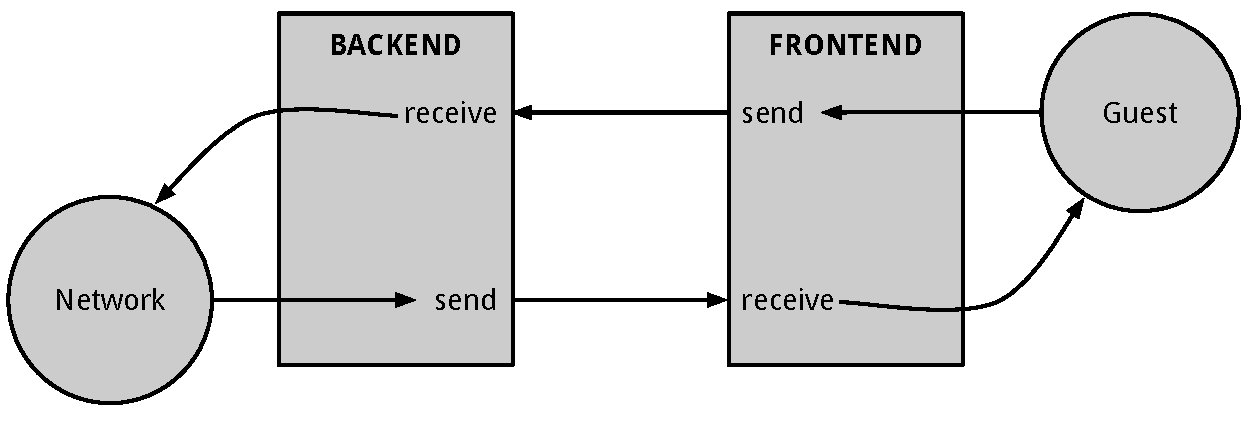
\includegraphics[scale = 0.60]{frontend-backend.pdf}
\caption{Interface between network frontend and network backend.}
\label{fig:frontback}
\end{figure}



\section{The e1000 class of network adapters}
\label{sec:e1000-hardware}
In this section we will illustrate some features and some details about the inner working of an e1000 ethernet network adapter.
Once again, we will only describe those aspects that are relevant to our goals.
The complete specification can be found in \cite{ref:e1000}.

\vspace{0.5cm}

Since the network communication is extremely important in the IT world, the market constantly pushes hardware vendors to produce high
performance, low-power, fully featured flexible, network adapters.

As a result, modern network devices are very complex. To get an idea of this complexity, one can observe that a device can implement 
more then a hundred of software-visible registers. Complexity is the price to pay in order to get high flexibity and several useful
features. Flexibility helps the IT administrator to tune the device parameters in order to find the right tradeoff between performance and 
power consumption, throughput and latency, and the like.
The rich set of features the device come with helps to adapt the device to different usage patterns and allows for performance 
optimizations (expecially for TCP/IP traffic) when offloading capabilities are present.
Hardware offloading features are supported by virtually every recent network adapter.

The most common feature are
\begin{itemize}
    \item Checksumming offload. When this feature is present, the device computes in hardware the checksums required by the main Internet 
	  protocols, such as IP, TCP and UDP. This saves the OS to do this work in software, which could be very expensive, expecially 
	  with checksums that are computed also on the payload and not only on the protocol header (e.g. TCP and UDP checksums).
	  
    \item TCP Segmentation Offload. When this feature is present, the device is able to do the TCP segmentation in hardware, splitting
	  a TCP segment over multiple ethernet frames. The segmentation is necessary because the real MTU of a TCP connection is almost
	  never greater than 1500 bytes (the ethernet original MTU), but the TCP window is commonly greater than that value. The OS
	  is then forced to do the splitting. With the feature present, however, the OS can send to the device driver a frame containing a 
	  TCP segment which is greater than the MTU\footnote{Up to 64KB with the Linux kernel.}. The device driver can pass that frame to
	  the adapter that performs the segmentation in hardware and sends multiple ethernet frames.
	  Apart from the obvious speed-up obtained because the operation is done in hardware rather then in software, this mechanisms has 
	  an important positive side effect. The network overhead necessary to traverse the TCP/IP stack is suffered only once, for a
	  big TCP packet, instead of once for each MTU-sized fragment. This clearly amortize the kernel per-packet overhead.
	  
    \item Scatter-gather capability. When this feature is present, the device is able to send a frame that is stored in multiple non
	  contiguous fragments in the machine physical memory. Therefore the OS is not forced to linearize (gather) the fragments,
	  avoiding the copy overhead. This is useful specially when the OS wants to send large packets. In other words the device is 
	  gather-capable.
\end{itemize}
The e1000 adapters have this three offloading capabilities.


\subsection{Data interface with the driver}
\label{sec:e1000-interface}
Being high performance devices, modern network adapters rely on Direct Memory Access (DMA) operations and interrupts.

When the device driver wants to send an ethernet frame through the adapter, it has to tell the adapter where the frame is stored
in physical memory and how long it is\footnote{When dealing with fragmented frames, the driver has to specify somehow a scatter-gather
array.}. Once the device knows where the frame is, it can directly access the physical memory\footnote{In this example we assume
there isn't any IOMMU.} and send it on the wire. More commonly, the frame is DMA'ed into an internal buffer for further processing before
being sent on the wire, but this is just a detail.

When the adapter receives a frame from the wire, it has to store it in the machine physical memory. For this reason, the device driver
has to tell the adapter where it can store incoming frames, before the frames actually comes. If the adapter doesn't know where to put
incoming frames, it cannot accept them.

\vspace{0.5cm}

It is clear that there must be a well-defined interface between the driver and the device. This interface is known as \emph{ring}.
A ring is a circular array of \emph{descriptors} that are used to exchange address/length information\footnote{Being an array a ring is a 
contiguous zone in the physical memory.}. A network adapter has at least two rings.
The first one is the \emph{TX ring} and it is used with outgoing frames, whereas the second one, the \emph{RX ring}, is used with
incoming frames. Network adapter can have multiple TX/RX rings with possibly different policies and priorities, so that one can
do some traffic engineering.

However, the e1000 adapter model emulated by QEMU has one TX ring and one RX ring. The array length, namely the number of descriptors,
can be chosen by the driver. In e1000 it must be a power of two and not more than 4096.


\subsubsection{TX ring}
\label{sec:txring}
The e1000 TX ring is an array of $N$ TX descriptors. Each TX descriptor is 16 bytes long and contains the address (in physical memory) and the
length of a frame (or a frame fragment) that is going to be sent or that has already been sent. The descriptor contains also flags that
can be used to specify options, and status bits. 

Two index registers are implemented for the synchronization between the driver and the adapter:
The TDT register (Transmit Descriptor Tail) and the TDH register (Transmit Descriptor Head). These are \emph{index} registers since
their value are array indexes with respect to the TX ring.

\vspace{0.5cm}

At the start-up, TDT and TDH are initialized by the driver to the same value, usually 0. When the driver wants to send a new frame,
it writes the physical address and the length of the frame in the TX descriptor pointed by the TDT register and then increments the TDT
register itself. Since the descriptor array is circular, the TDT must be set adequately.

When the adapter recognizes that TDH is different by TDT, is knows that there are new frames to transmit, and start processing the
descriptor pointed by TDH. A write access to the TDT register is therefore the way the device driver notifies the adapter that 
there are new frames ready to be sent.

For each descriptor to process:
\begin{enumerate}
  \item The frame pointed by the decriptor is sent on the wire.
  \item The TX descriptor is written back in order to set the DD (Descriptor Done) bit that indicates the TX descriptor has been
	processed.
  \item The TDH register is incremented circularly.
\end{enumerate}
The adapter stops the processing only when TDH == TDT, e.g. there are no more descriptors to process.

When the driver increments the TDT, the descriptor previously pointed (the one that has just been written) is committed to the hardware,
and the hardware owns it until the decriptor is processed.

Therefore, in each moment the ring is partitioned in two contiguous parts: The descriptors owned by the hardware, which are waiting
to be sent on the wire, and the descriptors owned by software, which are free to be used by the driver to commit new frames.

In order to prevent the index registers to wrap around, the driver should never use a TX descriptor if this is the very last free
TX descriptor. This happens when TDT is shuch that incrementing it circularly would cause TDT == TDH. When the TX ring is in this
state (TX ring full), the driver should stop transmitting. The transmission can be enabled again when the hardware process some descriptors,
incrementing TDH.

The figure \ref{fig:txring} depicts the TX ring with its index registers.

\begin{figure}[bt]
\centering
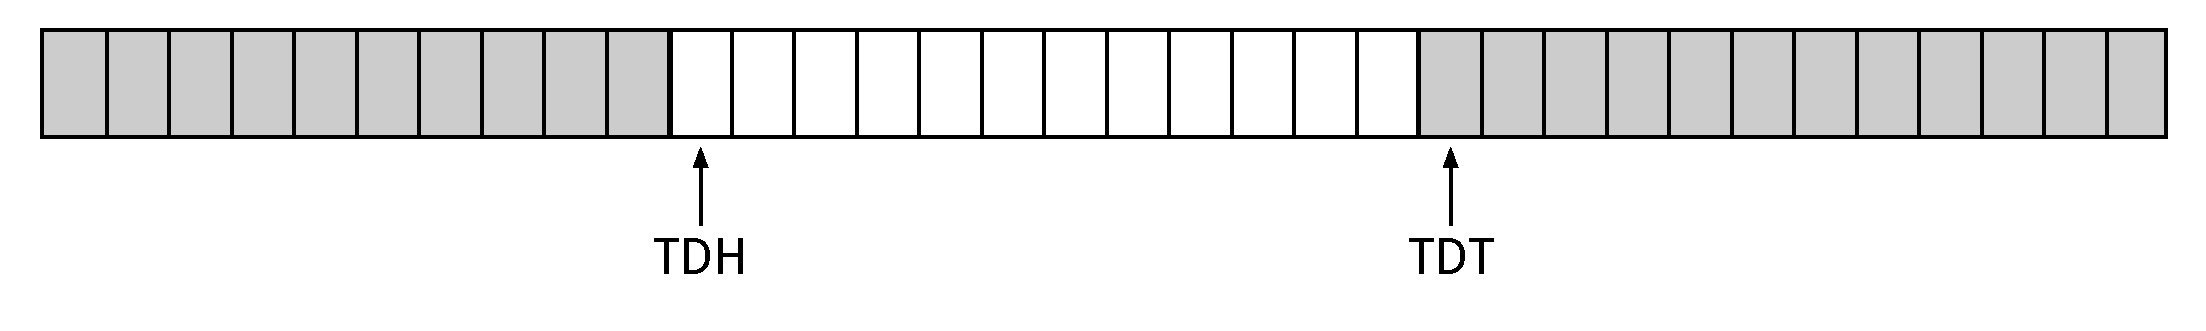
\includegraphics[scale = 0.35]{tx-ring.pdf}
\caption{The e1000 TX ring with its index registers. The grey area contains software-owned descriptors, while the white area
	contains hardware-owned descriptors.}
\label{fig:txring}
\end{figure}

\paragraph{Multi-descriptor frames}
Sometimes a frame is not stored contiguously in physical memory, or it's bigger than 4KB. In these cases the frame to transmit cannot
be specified with a single TX descriptor, but many consecutive TX descriptor must be used. The last TX descriptor describing a frame
must have the EOP (End Of Packet) bit set.

\paragraph{Context descriptors}
There are actually two generations of TX descriptors: Legacy descriptors and Extended descriptors, the latter being the most
recent ones.
When extended descriptors are used (this is normally the case), hardware offloading requests can be specified for each TX frame to send
by putting a so called \emph{context} descriptor in the TX ring before inserting the regular data TX descriptor(s).
Linux device driver makes use of extended TX descriptors and context descriptors.


\subsubsection{RX ring}
\label{sec:rxring}
The e1000 RX ring is an array of $N$ RX descriptors. Each RX descriptor is 16 bytes long and contains the address (in physical 
memory) and the length of a frame that has been received by the adapter, or only the address of a memory location that can be
used by the adapter to store an incoming frame. The descriptor contains also flags that can be used to specify options and status bits.
Two index registers are implemented for the synchronization between the driver and the adapter:
The RDT register (Receive Descriptor Tail) and the RDH register (Receive Descriptor Head). These are \emph{index} registers since
their value are array indexes with respect to the RX ring array.

\vspace{0.5cm}

At the start-up, the driver initializes RDH and RDT to 0. At this point, the adapter still doesn't know of any memory buffer where it
can store incoming frames, so it cannot receive anything.
To give the hardware memory buffers to work with, the driver puts the physical address of a memory buffer\footnote{How the memory 
buffer is allocated depends on the OS and on how the driver is implemented.} in the RX descriptor pointed by RDT and increments 
RDT circularly. Writing to the length field of the RX descriptor is useless, since this value is not used by the device. It's important to
note that the size of the memory buffer must be greater or equal then the maximum frame length, since we cannot know in advance how long
a future incoming frame is going to be.

A write access to the RDT register is therefore the way the device driver notifies the adapter that there are new memory buffers ready
to be used to store incoming frames.

If the adapter sees that RDH is different by RDT, it recognizes to have memory buffers available, and starts accepting incoming frames.
When a new frame arrives from the wire, the adapter
\begin{enumerate}
    \item Fetches the RX descriptor pointed by the RDH register.
    \item Copies the frame to the address contained in the RX descriptor.
    \item Writes back the descriptor in order to write the length of the received frame, and to set the DD (Descriptor Done) bit.
	  The DD bit indicates that the RX descriptor has been used to receive a frame.
    \item Increments the RDH register circularly.
    \item If programmed to do so, the device would normally sent an interrupt (see section \ref{sec:e1000int}), in order to tell
the driver there are new received frames ready to be pushed to the kernel network stack.
\end{enumerate}

When the driver increments the RDT, the descriptor previously pointed (the one that has just been written) is committed to the hardware,
and the hardware owns it until the decriptor is used.

Therefore, in each moment the ring is partitioned in two contiguous parts: The descriptors owned by the hardware, which can be
used to store new incoming frames, and the descriptors owned by software, which are unused or point to received frames ready to
be pushed to the network stack.

Similarly to what happens the TX ring, in order to prevent the register indexes to wrap around, the driver should never increment the RDT
register if the increment would cause RDT == RDH. When this situation happens (full RX ring) the driver should stop giving memory buffers to
the adapter. When new frame are received, the hardware increments RDH, and so it is possible to increment RDT again.

\vspace{0.5cm}

The interrupt routine should then push the arrived frames to the kernel and provide the adapter with more memory buffers (incrementing
the RDT), otherwise the adapter cannot accept more incoming frames.
A common strategy is to try to keep the RX ring always full. In order to do this, at the startup
the driver writes $N-1$ RX descriptor with the address of $N-1$ memory buffers, and set RDT to $N-1$, so that the ring is full.
Every time an interrupt arrives, the interrupt routine pushes the received frames to the kernel and replenish the ring, making it full again.
This strategy avoid situations in which the adapter is forced to reject incoming frames because it has no memory buffers available.

The figure \ref{fig:rxring} depicts the RX ring with its index registers.

\begin{figure}[bt]
\centering
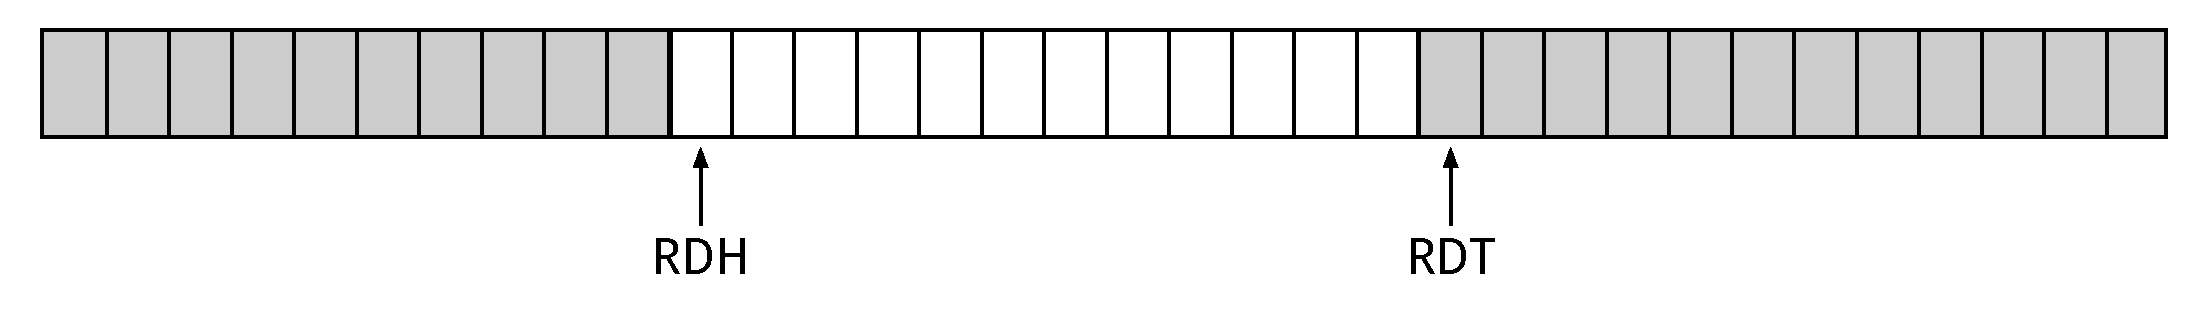
\includegraphics[scale = 0.35]{rx-ring.pdf}
\caption{The e1000 RX ring with its index registers. The grey area contains software-owned descriptors, while the white area
	contains hardware-owned descriptors.}
\label{fig:rxring}
\end{figure}


\subsection{Interrupts generation}
\label{sec:e1000int}
The e1000 network adapter can generate interrupts for different reasons, but we are interested in two types of interrupts:
\begin{itemize}
    \item TX interrupts: these interrupts are generated when the transmission of one ore more hardware-owned frames completes. Each TX 
	  descriptor has
	  a bit flag (Report Status, RS) that can be set to specify if the hardware has to send an interrupt as soon as the transmission 
	  of the associated
	  frame is complete. In every case an interrupt is always sent when the TX ring becames empty (TDH == TDT).
	  The interrupt routine, depending on the OS and the driver implementation, may execute cleanup operations on the descriptors 
	  that have been processed and mark them as free so that they can be used to commit new frame to the adapter.
	      
    \item RX interrupts: these interrupts are generated after the hardware has received (and stored in physical memory) an incoming frame, 
	  in order to notify the driver that it can send the frame to the kernel network stack. When the frame is sent to the kernel, it
	  will find the right way to its destination, that can be anything (trash included). Assuming the destination is a user process,
	  what the OS does is just appending the packet to a queue associated to the receiving socket. At this point the sleeping user
	  process is notified and can be scheduled to complete the read operation from the socket queue.
\end{itemize}

There is a big concern when dealing with RX interrupts. If the device doesn't limit them, they act as a source of uncontrolled load for the 
CPU.
The receiving machine, in fact, is forced to serve incoming RX interrupts even if the RX interrupt rate is very high. Since we are
dealing with high performance devices, we would like to be able to receive up to 1 Mpps (or even more).
The overhead involved in interrupt handling is generally quite high, and so each interrupts has a fixed cost that must be paid before
doing useful work, such as push the received frame to the network stack and let the receiver process actually receive it.

If each packet receive generated an interrupt, we would have to handle up to 1000000 interrupts per seconds, which something that would
completely stall our machine.
When the interrupt rate is too high, in fact, the machine spends almost all the time serving interrupts\footnote{The interrupt handling is
by its nature an high priority task with respect to normal process execution.}, and there is no time left for other things to happen,
e.g. for user processes to read the received packets. This is a quite bad situation, because the CPU is 100\% utilized, but the machine,
on the whole, cannot do any useful work (this is the \emph{livelock} problem).

The situation could be slightly better if the machine has more than one CPU, but still it's not good for the CPU servicing the interrupts
to spend too much time in interrupt handling overhead.

\vspace{0.5cm}

Cleary, this problem can only be solved if the device somehow collapses RX interrupts, raising an interrupt every batch of received
frames, let's say 100 frames per batch, and not every single frame. In this way the interrupt rate is 100 times lower, and the
interrupt overhead cost is amortized over 100 frames.
In every case the device must guarantee that a RX interrupt is eventually sent after a period of inactivity, even if it is still waiting
for a 100-frames batch to be completed, because the device cannot know when the next frames are going to come.

These and similar mechanisms are known as \emph{interrupt mitigation} or \emph{interrupt moderation}, since they tries to moderate the
interrupt rate.

Interrupt moderations is commonly applied also to TX interrupts (or to all the interrupts in general). The TX interrupt rate can be
controlled because the driver can control (and limit) the TX rate. Neverthless it is convenient for the driver to take advantage of
the interrupt-rate-limiting hardware capabilities rather than implement a similar feature in software\footnote{With e1000, an TX 
interrupt moderation mechanism could be implemented using the RS bit.}.

\vspace{0.5cm}

The e1000 class of network adapters implements two interrupt moderation mechanisms.

\subsubsection{The older moderation mechanism}
\label{sec:oldmit}
The older mechanism is supported by the registers TIDV (Transmit Interrupt Delay Value), TADV (Transmit Absolute Interrupt Delay Value),
RDTR (Receive Delay Timer Register) and RADV (Receive Interrupt Absolute Delay Value), where each register is provided with a countdown
timer.

\vspace{0.5cm}

TIDV and TADV, when properly set, can be used to provide TX interrupt moderation on a per-descriptor basis.

When the adapter processes a a TX descriptor, if the RS bit and the IDE bit\footnote{The Interrupt Delay Enable bit (IDE), is another
bit flag in the TX descriptor, like the RS bit.} are set, an interrupt is not raised immediately, but the TIDV timer is armed (or
rearmed) with the value specified in the TIDV register itself. When the TIDV timer expires, an interrupt is raised in order
to inform the driver about the TX completion of one or many frames.
The TIDV register can therefore be used to coalesce TX interrupts.

However, it might be necessary to ensure that no completed transmission remains unnoticed for too long an interval in order to 
ensure timely release of TX buffers.
The TADV register has been added for this purpose. Like the TIDV timer, tha TADV timer only applies to TX descriptor where both the
RS bit and the IDE bit are set. This register can be used to ensure that a TX interrupt occurs before a predifined time interval
after a transmission (whatever) is completed. The time interval can be specified in the TADV register itself.
After each TX descriptor is processed, the TADV timer is is armed with the value specified in the TADV 
register only if it is not already running.
When the timer expires, a TX interrupt is generated.

\vspace{0.5cm}

RDTR and RADV, when properly set, can be used to provide RX interrupt moderation on a per-received-frame basis.
The RDTR timer is armed (or rearmed) immediatly after a new packet is received and transferred to physical memory, using
the interval value specified in the RDTR register. When the RDTR timer expires, an RX interrupt is raised, and the timer is cleared.
The RDTR register can therefore be used to coalesce RX interrupts, in the very same way the register TIDV is used to coalesce TX
interrupts.

Also in the RX case it may be necessary to ensure that no receive remains unnoticed for too a long interval. The RADV register deal
with this problem, in the very same way the TADV register does, so we won't explain the mechanism again.

\vspace{0.5cm}

Figure \ref{fig:rdtrstate} shows a state diagram associated to the RDTR timer, while figure \ref{fig:radvonly} depicts an example
about the RADV moderation mechanism.

\begin{figure}[bt]
\centering
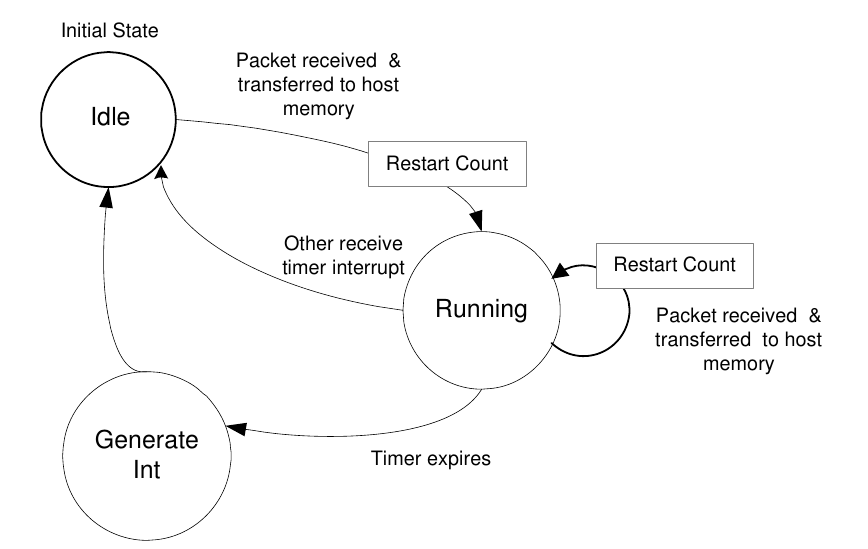
\includegraphics[scale = 0.45]{rdtr-state.png}
\caption{State diagram of the RDTR timer (Packet Delay Timer). CITE INTEL}
\label{fig:rdtrstate}
\end{figure}

\begin{figure}[bt]
\centering
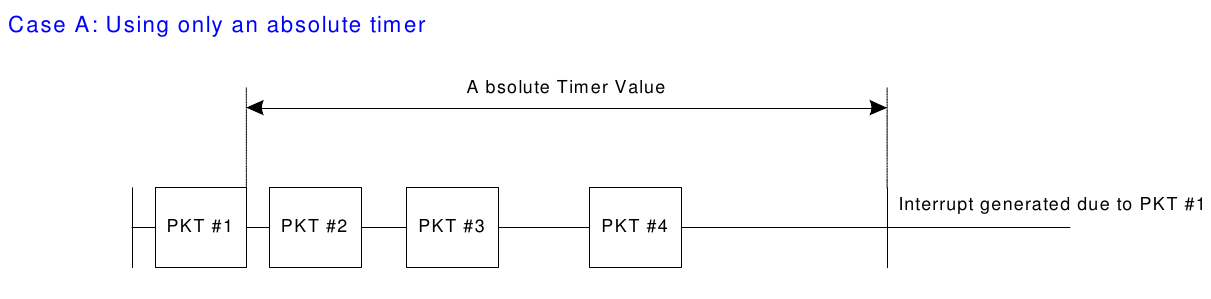
\includegraphics[scale = 0.45]{radv-only.png}
\caption{RX moderation example that makes use of the RADV timer.}
\label{fig:radvonly}
\end{figure}

\subsubsection{The newer moderation mechanism}
\label{sec:itrmit}
Although the older mechanisms allows for fine grained control over the moderation, especially on the TX side, most of the times the 
required moderation functionality is way simpler. For this reason a more direct moderation mechanism has been added, which is implemented
through the ITR register (Interrupt Throttling Register).

If the driver sets this register to a value $\delta$, the board ensures that $\delta$ is the minimum inter-interrupt interval, regardless of
network traffic condition, and the interrupt type.
In other words, every time an event happens that requires an interrupt (e.g. TX completion or RX completion) the board raise an interrupt
as soon as possible, while meeting the ITR inter-interrupt delay constraint.

\vspace{0.5cm}

The ITR mechanism, when used, applies to all the interrupts. The Intel manual strongly recommend avoiding the RDTR and RADV register,
and use the ITR instead.



\section{QEMU e1000 emulation}
\label{sec:e1000emu}
The e1000 frontend is implemented in QEMU through a single source file\footnote{hw/e1000.c in the QEMU project root directory} (see 
section \ref{sec:frontback}).

A small part of this code contains declarations and routines necessary to register and initialize/uninitialize a new type of PCI Ethernet 
device within the rest of the emulator. In this way one or more instances of the e1000 network device can be included in a VM
when launching QEMU\footnote{This is done through the \texttt{device} option. E.g. \texttt{qemu-kvm -device e1000 ...} }.

When registering a new PCI device, it is necessary to describe the I/O or MMIO regions that the device implements, registering new
PCI BAR registers. Each BAR register correspond to a different I/O or MMIO region.
When registering a new BAR, you can specify two callback functions that are invoked whenever the guest code access (reads or writes)
a location in a region.

The e1000 emulation code registers a MMIO region and an I/O region. The I/O region isn't actually used, whereas
the MMIO region maps all the registers the e1000 device implement, such as TDT, TDH, RDH and so on.

A couple of statically defined dispatch tables, one for the read accesses and the other for the write accesses, are used to associate a
different function to each register.
In this way one can (potentially) associate a different read callback and a write callback to each e1000 register.
The emulation of a device is basically achieved with this per-register functions. Of course register can share the same functions or have
no callbacks at all.

\vspace{0.5cm}
Let's see in more depth how register callbacks are actually invoked.

When a VCPU is executing the guest code, it may try to access a MMIO location corresponding to the e1000 PCI device, namely an e1000
register. This usually happens when executing the e1000 device driver.
The accessing instruction causes a VMExit to occur, and the VCPU thread switches from the guest world to the host world. 
After the \texttt{iothread lock} has been acquired, the QEMU code analyzes the VMExit reason and understands that the VMExit was caused
by a MMIO access.
It then uses the physical memory address involved in the MMIO access to dispatch the event to the right PCI memory region.
In our case, the read (write) callback registered with the e1000 MMIO BAR is invoked. This callback uses the address to access the 
e1000 read (write) dispatch table and invokes the register-specific callback.

The register-specific callback emulates the side effects associated with the register access. For instance a write to the TDT
register will cause the emulated hardware to process all the pending TX frames (see section \ref{sec:txring}).

After the callback returns, the \texttt{iothread lock} is released and a VMEnter is executed so that the VCPU switches back to the 
guest world.

\vspace{0.5cm}

This said, we won't describe in detail all the aspects involved in e1000 emulation. Instead, we will outline the frame
transmission and frame reception process, focusing on notifications, scheduling and memory copies.


\subsection{TX emulation}
\label{sec:e1000txemu}
As stated in section \ref{sec:txring}, a write to the TDT register is the way the driver notifies the hardware that new TX frames 
are ready to be processed.
The TDT register write callback updates the TDT value and then calls the \texttt{start\_xmit} function. This function is a while
loop that processes all the committed TX descriptors, starting from the descriptor pointed by the TDH register. After each
descriptor is processed, the TDH register is incremented circularly. The while loop exits when TDT == TDH, e.g. when there
are no pending TX descriptors.

\vspace{0.5cm}

TX descriptors processing includes the following actions:
\begin{enumerate}
    \item The TX frame corresponding to the TX descriptor is copied from the guest memory to a local buffer.
    
    \item The TCP/UDP checksum is computed. Recall that e1000 devices are able to compute checksums in hardware, and so the OS 
	  driver expects the emulated hardware to be able to do it.
	  
    \item The \texttt{qemu\_send\_packet} function is invoked in order to pass the frame to the network backend. With the TAP backend,
	  a \texttt{write} system call is invoked to pass the frame to the TAP device associated with the backend.
	  
    \item The descriptor is written back to the guest memory in order to report that the TX descriptor has been processed.
\end{enumerate}

When all the pending TX descriptors have been processed, the interrupt pin associated with the e1000 adapter is raised (if the previous
pin state was low), sending an interrupt to the guest. The interrupt moderation registers (see section \ref{sec:itrmit}) are not implemented.

\vspace{0.5cm}

It's very important to observe that all these operations (frontend and backend) are performed by the same VCPU thread that tries to 
execute the TDT write operation in the guest, causing a VMExit.
This means that when the guest has only a VCPU (no SMP) the emulation of a transmission cannot be done in parallel with the guest, being
done synchronously with the VCPU thread.



\subsection{RX emulation}
\label{sec:e1000rxemu}
When a receiving guest is waiting for new frames to come, the IOThread is blocked in the \texttt{select} system call, waiting for
the TAP file descriptor to be ready.
When a frame arrives to the TAP backend, the \texttt{select} returns and invokes the TAP network backend.
The backend executes a \texttt{read} system call on the TAP device, extracting the incoming frame, and invokes the
\texttt{qemu\_send\_packet} function that passes the frame to the e1000 frontend, invoking the \texttt{receive} method
(\texttt{e1000\_receive}).

\vspace{0.5cm}

According to what has been presented in section \ref{sec:rxring}, the \texttt{e1000\_receive} method performs the following actions:
\begin{enumerate}
    \item If RDH == RDT, there are no RX memory buffer available, and the incoming frame must be dropped. Otherwise go to step 2.
    \item The RX descriptor pointed by the RDH register is fetched from the guest memory.
    \item The incoming frame is copied to the guest memory location at the address specified in the RX descriptor.
    \item The RX descriptor is written back to guest memory, in order to report the length of the received frame and set the DD bit.
    \item If not already high, the e1000 interrupt pin is raised.
\end{enumerate}

Differently from the TX emulation, here all these operations (frontend and backend) are executed by the IOThread, that can run in parallel
with the VCPU thread (or the VCPU threads) executing the guest code.

\vspace{0.5cm}

When the \texttt{qemu\_send\_packet} function returns, the backends tries to read another frame from the TAP\footnote{The \texttt{read}
system call is non-blocking, since the IOThread is executing an event-loop, and so only the central \texttt{select} system call is
allowed to block.}. If there is another frame to process, the \texttt{qemu\_send\_packet} is called also on this frame.
This process stops when no frames are ready to be read from the TAP, or when the packet is dropped by the frontend.



\section{Linux e1000 device driver}
\label{sec:e1000driver}
In this section we will describe some details about the e1000 device driver in the Linux kernel, which is implemented as
a kernel module.
We will only illustrate those aspects that are relevant to our goals.
The driver source code can be found in the directory \texttt{drivers/net/ethernet/intel/e1000} in the Linux kernel project root directory.

\subsection{Interface with the network stack}
\label{sec:netapi}
The Linux kernel API has a specific network API that the network device drivers use to exchange network packets with
the rest of the kernel.

With these API, the network driver can register a new network interface within the kernel, associating a name to it.
The list of all the network interfaces currently registered within the kernel can be seen using the \texttt{ifconfig} utility
(e.g. \texttt{\$ ifconfig -a}) or similar tools.
The registering function, \texttt{register\_netdev}, requires as input argument a \texttt{netdev} structure that abstracts the
registering network adapter. This structure contains all the information necessary to the kernel to communicate with the adapter.

\vspace{0.5cm}

The most important \texttt{netdev} fields are:
\begin{itemize}
    \item \texttt{name}, which is a string that univocally identifies the new network interface in the system.
    
    \item \texttt{netdev\_ops}, which is a structure containing the methods that the new network interface exports to the kernel 
	  (see below).
	  
    \item \texttt{watchdog\_timeo}, which specifies the minimum time interval that the kernel should wait after a transmission is commited
	  to the device driver before deciding that something could be wrong. When a transmission is committed, the watchdog timer 
	  associated with the network interface is started. When the driver knows that the hardware it done with the committed frame,
	  it release the associated TX buffer (in e1000 this can be done in the routine that handles the TX interrupt). On the release,
	  the watchdog timer is cleared. If the timer fires, the \texttt{ndo\_tx\_timeout} method is called, so that the driver can
	  handle potential hardware hangs.
	  
    \item \texttt{hw\_features}, which is a bitmask that specifies to the kernel the features offered by the hardware that can be activated
	  or deactivated by the user. The e1000 device driver specifies, among the others, the \texttt{NETIF\_F\_HW\_CSUM} (checksumming
	  capability) feature, the \texttt{NETIF\_F\_SG} (scatter-gather capability) feature and \texttt{NETIF\_F\_TSO} (TCP Segmentation
	  Offload capability).
	  
    \item \texttt{features}, which is a bitmask that represent the currently active features. This mask can be initialized to the same
	  value as the \texttt{hw\_features} field, but can be modified by the users to set/unset features and is fixed by the kernel in
	  order to meet feature constraints\footnote{The features are not independent on each other within the kernel.}.
	  
    \item \texttt{dev\_addr} and \texttt{perm\_addr}, which contain the hardware address of the network adapter. As far as we are
	  concerned, these two fields are set to the same value. In the e1000 adapter, the hardware address is read from an on-board
	  EEPROM.
\end{itemize}


The \texttt{netdev\_ops} contains several methods, but we are intersted only in a few ones:
\begin{itemize}
    \item \texttt{ndo\_open}, which is called when the system administrator decides to bring the network interface up. This can be done
	  using the \texttt{ifconfig} utility (e.g. \texttt{\#ifconfig eth0 up}) or similar. The driver should react to this request by
	  setting up all the resource (software or hardware) necessary for the adapter operation. The e1000 \texttt{ndo\_open} method
	  allocates and initializes all the resource necessary for TX/RX operation (e.g. RX and TX rings), initializes the registers,
	  enables the e1000 interrupts and invokes the \texttt{netif\_start\_queue} function, which tells the kernel it can start invoking
	  the \texttt{ndo\_start\_xmit} method (see below).
	  
    \item \texttt{ndo\_close}, which is called when the system administrator decides to bring the network interface down, This can be
	  done using the \texttt{ifconfig} utility (e.g. \texttt{\# ifconfig eth0 down} or similar). When receiving this request,
	  the driver can release all the resource allocated by the \texttt{ndo\_open} method.
	  
    \item \texttt{ndo\_start\_xmit}, which is invoked by the kernel when it wants to transmit a new frame. The first argument is
	  a pointer to a \texttt{sk\_buff} structure, which contains all the information related to the frame to transmit, including
	  the frame itself. The \texttt{sk\_buff} structure is central to the Linux kernel networking, since all the layers in the 
	  network stack perform actions on this structure.
	 
\end{itemize}

On the receive side, the kernel networking API provides the network driver with a function (\texttt{netif\_rx()}) for passing a
received frame up to the network stack, where the frame can find its way to its destination.
The frame is handed off to the network stack in a \texttt{sk\_buff} structure.
When receiving a frame from the adapter, therefore, the driver has to build a \texttt{sk\_buff} structure around the frame received
and call the function \texttt{netif\_rx()} with the structure built as parameter.

\begin{figure}[bt]
\centering
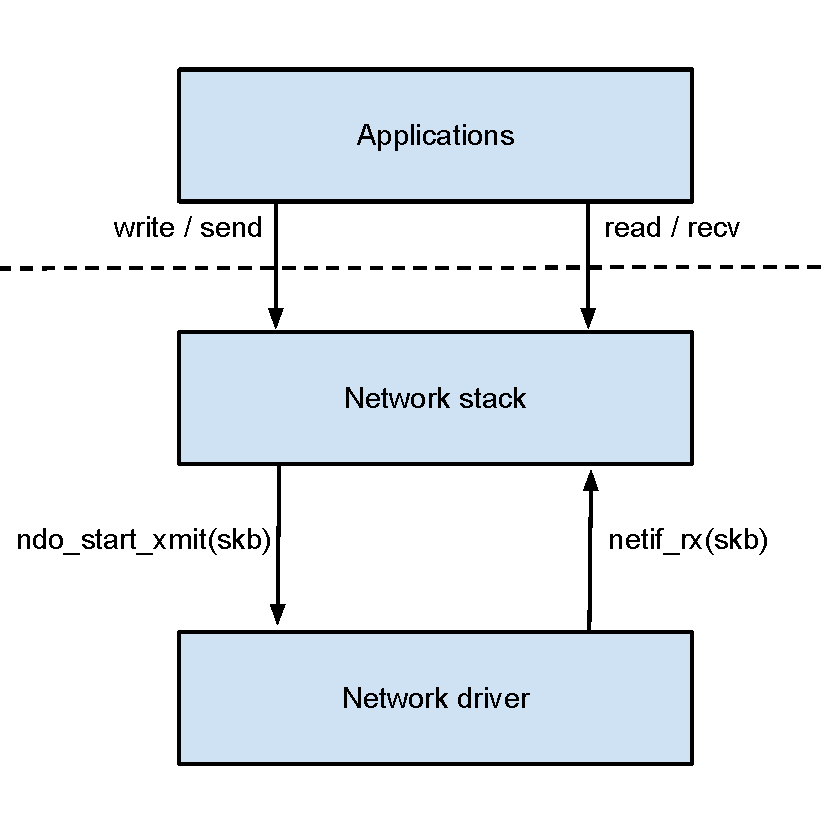
\includegraphics[scale = 0.65]{linux-interface.pdf}
\caption{On the bottom the interface between the network device driver and the network stack, and on the top the interface between
user applications and the network stack.}
\label{fig:linux-interface}
\end{figure}


\subsubsection{The NAPI interface}
\label{sec:napi}
The receive interface described earlier is known as the ``old'' interface. The \texttt{netif\_rx} is intended to be invoked
directly by the interrupt routine associated with an RX interrupt.

However, as we pointed out earlier (see \ref{sec:e1000int}), the RX interrupt are source on uncontrolled load and must be moderated when
the interrupt rate is too high. This can be done by hardware mechanisms, but a complementary software approach can still be useful.
Moreover, a software interrupt moderation can be fundamental if hardware moderation is not provided by the network adapter.

\vspace{0.5cm}

The software approach is based on the concept of \emph{polling}. Interrupt operation was introduced in the early days of computing when
the computer architects realized that when dealing with devices through polling most of the CPU cycles were thrown away because of
busy waiting. Interrupt operation makes it possible to avoid busy waiting, even if it carries with it a fixed overhead, due to the
context switches and scheduling/dispatch operations, that is fairly high.

Nevertheless, if there are (almost) always hardware I/O events to handle, busy waiting is not a problem, since there is (almost) nothing to
wait for.
Polling can therefore be used in those situations where the input load is very high, since each time we want to check if there are more 
hardware events to we are likely to find them. The big advantage of polling operation over interrupt operation is that the former does
not have any fixed overhead.

\vspace{0.5cm}

In conclusion, one cannot say in general that interrupt operation is better than polled operation or the other way around. When the hardware
event rate (e.g. frame reception rate) is low enough, it's worth paying the fixed cost associated with interrupts in order to be sure that
there is an event to handle. When the event rate is high enough, however, busy waiting it's cheaper than interrupts, because the average 
number of cpu cycles wasted to busy wait for the next frame is way lower than the cpu cycles wasted for the interrupt overhead.

\vspace{0.5cm}

The NAPI (New API) interface has been designed with these considerations in mind. When a RX interrupt arrives, the driver interrupt routine
can decide to switch to polling mode, and not to handle the received frame directly.
This is done simply disabling the interrupt on the network adapter and scheduling a NAPI context. The latter action is done invoking the 
function \texttt{napi\_schedule}.
The NAPI context is going to be executed in a kernel thread context different from the interrupt context: This is basically another form
of deferred work.

When the NAPI context is scheduled it executes the NAPI polling function registered by the driver through the function 
\texttt{netif\_napi\_add} (this function registration could be done in the \texttt{ndo\_open} method).

The NAPI polling function is in charge of doing the receive work\footnote{or the interrupt work in general}. Of course the polling function
is intended to process more RX frames. In order to prevent the polling function to monopolize the CPU, however, there must be a limit on 
the work done by the polling function. This is the reason why the polling function is invoked with a \texttt{budget} input argument, that
specifies the maximum number of RX frames to process.
If the budget is comsumed entirely, the polling function should return, so that the NAPI context will be rescheduled in the future: However,
the interrupts are not enabled. In these way the NAPI keep polling the device as long as there is RX work to do.

If the budget is comsumed only partially, however, the polling function should assume that it's not worth polling again, and switches back
to interrupt operation. This is done calling the \texttt{napi\_complete} function, and then reenabling the adapter interrupts. The NAPI
context won't be scheduled again until the next interrupt routine calls the \texttt{napi\_schedule} function the next time.

\vspace{0.5cm}

In the end, with the NAPI interface the driver is able to switch between interrupt operation an polled operation depending on the current
incoming traffic conditions, providing a form of interrupt moderation that can greatly increase the receive throughput.

The e1000 driver currently use the NAPI interface instead the older one.


\subsection{Interface with the PCI subsystem}
Since an e1000 network adapter is a PCI device, the first thing the driver has to do when the e1000 kernel module is loaded is 
registering a new PCI driver within the kernel PCI subsystem. The registration is done through the function \texttt{pci\_register\_driver},
which accepts a \texttt{pci\_driver} structure as input argument.
The \texttt{pci\_driver} structure contains all the information useful to the Linux PCI subsystem to manage the PCI device.

\vspace{0.5cm}

The most important fields of the \texttt{pci\_driver} structure are:
\begin{itemize}
    \item \texttt{id\_table}, which is a list of all the PCI devices managed by the driver. A PCI device is identified by
	  a vendor ID and a device ID.
    \item \texttt{probe}, which is a method that the PCI subsystem invokes when it detects (e.g. by PCI enumeration) that a new PCI
	  device is attached to the PCI bus. The PCI subsystem invokes the probe method of the driver that manages the specific PCI device
	  detected. The e1000 probe method initializes, configures and reset the board, an then registers a new network interface (see
	  section \ref{sec:netapi}).
    \item \texttt{remove}, which is a method that the PCI subsystem invokes to alert the driver that it should release the PCI device,
	  because of a Hot-Plug event or because the driver is going to be removed from memory. The e1000 remove method undo all the
	  operations done by the e1000 probe method, disabling the adapter operation.
\end{itemize}

Once the PCI subsystem invokes the e1000 probe method, a new e1000 network interface is registered within the kernel and is ready to be
used.


\subsection{TX operation}
\label{sec:txdriver}
As outlined in section \ref{sec:netapi}, when the network stack decides to send a packet through the e1000 adapter, the e1000
\texttt{ndo\_start\_xmit} method is invoked. What the driver has to do is extracting the frame data and other useful information from the 
input \texttt{sk\_buff} structure, and commit the frame to the adapter. The first byte of the frame is stored at the address contained
in the \texttt{data} field of the structure.

The input \texttt{sk\_buff} can be \emph{linear} or \emph{non-linear}. If linear, the frame is a stored in a contiguous memory
area\footnote{Being kernel \emph{logic} addresses, the frame is contiguous both in virtual and physical memory.}.
If non-linear, the frame is not contiguous, but is stored as a collection of contiguous fragments (e.g. is specified by a scatter-gather
array).

\vspace{0.5cm}

In order to write the TDT register only when necessary, the driver has a shadow variable, \texttt{tx\_next\_to\_use}, that is intended to
be used in place of the TDT when possible. The TDT register is updated with the variable content only when the driver wants to commit a 
frame to the hardware. In this way is never necessary to read the TDT register, since one can read the shadow variable instead.

Similarly, there is a shadow variable, \texttt{tx\_next\_to\_clean}, also for the TDH register. The shadow variable is incremented
once for each used TX descriptor that has the DD bit set (see below). In this way it's never never necessary
to read the TDH register, since one can read the shadow variable instead\footnote{Recall that
the driver normally does not need to write the TDH register, except for register initialization.}.

Even though the driver wasn't written with virtualization problems in mind, these shadow variables are extremely useful, because 
accessing a register cause an expensive VMExit, while accessing memory is done at native speed.

\vspace{0.5cm}

Moreover, in order to keep trace of per-descriptor information that can be used to release the resources when the transmission is done, 
the driver mantains an array parallel to the TX ring, the \texttt{tx\_buffer\_info} array.
As an example, some elements in this parallel array contain a valid pointer to a \texttt{sk\_buff} structure passed by the kernel. Since
this structure (data included) is dynamically allocated, the driver has to free its memory, but only when it is sure that the frame 
contained has actually been sent on the wire. As we will see, this cleanup is done by the TX interrupt routine.

\vspace{0.5cm}

In more detail, the e1000 \texttt{ndo\_start\_xmit} method does the following:
\begin{itemize}
    \item Checks if there are enough free TX descriptors for the frame to send. If not, returns immediately reporting the adapter as busy.
          Since the \texttt{sk\_buff} can be non-linear, we have to use a different TX descriptor for each fragment. Moreover, an additional
	  context descriptor may be necessary in order to make a offload requests on the current frame (see \ref{sec:txring}).

    \item If necessary, inserts a new context descriptor in the TX ring location pointed by the \texttt{tx\_next\_to\_use} variable, and
	  increment the variable. The context descriptor refers to the following data TX descriptors.
	  The \texttt{ip\_summed} field in the \texttt{sk\_buff} structure says if the frame need to be checksummed. The \texttt{gso\_size}
	  field of the \texttt{skb\_shared\_info} structure associated with the \texttt{sk\_buff} says if the frame need TCP Segmentation
	  Offload.

    \item Maps all the frame fragments into DMA-capable physical memory (DMA mapping). The mapping is necessary to tell the kernel that
	  we are going to access the memory regions with DMA. The mapping function returns the physical addresses corresponding to a
	  fragment, and doesn't perform a copy. An entry of the \texttt{tx\_buffer\_info} array is used for each fragment to store
	  its physical address and length. A pointer to the input \texttt{sk\_buff} is stored in the entry corresponding to the last
	  fragment. Being the array parallel to the TX ring, the driver starts to use the entry pointed by the \texttt{tx\_next\_to\_use} 
	  variable (but don't increment the variable itself, since it will be incremented in the next step).
	  
    \item Inserts in the TX ring a data TX descriptor for each frame fragment, using the information just stored in the parallel array,
	  and incrementing \texttt{tx\_next\_to\_use} by the number of fragments.
	  
    \item Updates the TDT register with the \texttt{tx\_next\_to\_use} content, in order to commit the new frame to the hardware.
\end{itemize}

From the previous list follows that the driver needs to do some per-frame cleanup operations after the hardware has actually sent the
frame. This is the reason why TX interrupts are enabled. Therefore, after the hardware has sent one or more frames, it eventually 
raises an interrupt.

\vspace{0.5cm}

Since the e1000 driver uses the NAPI, the interrupt routine disables the e1000 interrupts and schedules the NAPI context.
The e1000 NAPI polling function, \texttt{e1000\_clean}, is (also) in charge of doing the TX cleanup work. This work is done invoking
the function \texttt{e1000\_clean\_tx\_irq}.

Starting from the entry pointed by \texttt{tx\_next\_to\_clean}, the polling function fetches the TX descriptors to see what descriptors
have the DD bit set, and so have been processed (used) by the hardware. For each used descriptor, it releases the TX resources using the
information stored in the corresponding entry in the parallel \texttt{tx\_buffer\_info} array. In more detail, the driver undoes the DMA
mapping of each data TX descriptor and frees the \texttt{sk\_buff} of the last data TX descriptor associated with each frame sent.


\subsection{RX operation}
\label{sec:rxdriver}
In order to access the RDT register only when necessary, the driver has a shadow variable, \texttt{rx\_next\_to\_use}, that is intended to
be used in place of the RDT when possible. The RDT register is updated with the variable content only when the driver wants to give new
memory buffers to the hardware. In this way is never necessary to read the RDT register, since one can read the shadow variable instead.

Similarly, there is a shadow variable, \texttt{rx\_next\_to\_clean}, also for the RDH register. The shadow variable is incremented
once for each used RX descriptor that has the DD bit set (see below). In this way it's never never necessary
to read the RDH register, since one can read the shadow variable instead\footnote{Recall that the driver normally does not need to write
the RDH register, except for register initialization.}.

Once again, the shadow variables are extremely useful to minimize the number of VMExits.

\vspace{0.5cm}

Similarly to what happens for the TX operation, the driver mantains an array parallel to the RX ring, the \texttt{rx\_buffer\_info} array,
in order to keep trace of per-descriptor information that can be used to release the resources when the reception is completed.
As an example, each entry in this parallel array contains the DMA-mapped physical address of a memory buffer used by the adapter to
receive a frame. The driver must undo the DMA-mapping, but only after the memory buffer has been used by the hardware.

\vspace{0.5cm}

When initializing the the resources for RX operation, the e1000 \texttt{ndo\_open} method also calls the \texttt{e1000\_alloc\_rx\_buffers()}
function passing $N-1$ as \texttt{cleaned\_count} input parameter, so that this function allocates $N-1$ memory buffers to be used for frame 
reception (see section \ref{sec:rxring}). In this way the adapter can accept incoming frames as soon as the reception is enabled in the 
hardware.

\vspace{0.5cm}

In more detail, for each buffer to allocate, the \texttt{e1000\_alloc\_rx\_buffers} function:
\begin{enumerate}
    \item Allocates a new \texttt{sk\_buff} structure that has enough data room to store a maximum size ethernet frame.
    
    \item Stores a pointer to the \texttt{sk\_buff} into the entry of the \texttt{rx\_buffer\_info} array indexed by the 
	  \texttt{rx\_next\_to\_use} content. In this way this pointer can be
	  passed to the network stack by the RX interrupt routine after the memory buffer contained into the \texttt{sk\_buff} itself
	  is used by the hardware.
	  
    \item Maps the memory buffer so that it can be accessed in DMA, similarly to what happens for TX frames (see section 
	  \ref{sec:txdriver}). The physical address of the memory buffer is stored in the same \texttt{rx\_buffer\_info} entry.
	  
    \item The buffer physical address is also written into the RX descriptor corresponding to the \texttt{rx\_buffer\_info} 
	  entry\footnote{Recall that the RX ring and the \texttt{rx\_buffer\_info} arrays are parallel}.
	  
    \item The \texttt{rx\_next\_to\_use} variable is incremented. If is the case (see below) the RDT register is then updated with the 
	  \texttt{rx\_next\_to\_use} content.
\end{enumerate}

A write to the RDT register is performed every 16 allocated memory buffers, and at end of the \texttt{e1000\_alloc\_rx\_buffers} function.

There is a tradeoff here: Writing the RDT at each iteration would be too slow, and writing the RDT only at the end of the function would
cause the receive side to be poorly reactive.

\vspace{0.5cm}

After one or more new frames are received and stored in the physical memory, an interrupt is eventually raised.
The interrupt routine disables the e1000 interrupt and schedules the NAPI context (see \ref{sec:txdriver}).
The e1000 polling function is (also) in charge of doing the RX work.

Though the e1000 adapters are able to receive also \emph{jumbo} frames\footnote{ethernet frames that can carry up to 9000 bytes of payload},
in the following we will describe only what happens when conventional ethernet frame are used\footnote{Anyway, the jumbo frame handling 
it's not very different.}.

In order to do the RX work, the e1000 polling function invokes the \texttt{e1000\_clean\_rx\_irq} function.
This function starts to fetch and clean used RX descriptors beginning from the one indexed by \texttt{rx\_next\_to\_clean}.
It keeps working while the NAPI budget is not exhausted and the descriptors have the DD bit is set. The latter indicates that the 
RX descriptor has been used by the hardware to receive a frame.

\vspace{0.5cm}

For each RX descriptor to clean:
\begin{enumerate}
    \item The used memory buffer is DMA-unmapped. The buffer physical address is taken from the \texttt{rx\_buffer\_info} entry
	  corresponding to the RX descriptor.

    \item If the received frame is shorter than 256 byte\footnote{This number is a kernel parameter that can be tuned by the user.},
	  the copybreak mechanism fires: A new minimum size \texttt{sk\_buff} structure is allocated and the frame data are copied,
	  while the old \texttt{sk\_buff} will be recycled. This should improve packet loss for small packets, because the socket
	  receive queues get full earlier if the enqueued \texttt{sk\_buff} are bigger.
	  
    \item Some fields of the \texttt{sk\_buff} structure built around the received frame are properly initialized\footnote{For example the
	  \texttt{ip\_summed} and the \texttt{protocol} fields.} and the frame
	  is handed off to the network stack (see the \texttt{e1000\_receive\_skb()}) function. A pointer to that structure is
	  taken from the same \texttt{rx\_buffer\_info} entry, if the copybreak mechanism did not fire.
\end{enumerate}


